\documentclass{acmconf}
\usepackage{graphicx}
\usepackage{multicol}
\usepackage{amssymb,amsmath,epsfig,alltt}
\sloppy
\usepackage{palatino}
\usepackage{pdftricks}
\begin{psinputs}
  \usepackage{pstricks}
  \usepackage{pst-node}
\end{psinputs}
\usepackage{parskip}
\usepackage{tabularx}
\usepackage{alltt}
\bibliographystyle{amsplain}

\title{\textbf{\textsf{
Complete Translation of Unsafe Native Code to Safe Bytecode
}}}
\date{}
\author{\begin{tabular}{@{}c@{}}
        {\em {Brian Alliet}} \\
        {Rochester Institute of Technology}\\
        {\tt bja8464@cs.rit.edu}
   \end{tabular}\hskip 1in\begin{tabular}{@{}c@{}}
        {\em {Adam Megacz}} \\
        {University of California, Berkeley} \\
        {\tt megacz@cs.berkeley.edu}
\end{tabular}}
\begin{document}

\maketitle

\begin{abstract}

Most existing techniques for using code written in an unsafe language
within a safe virtual machine involve transformations from one source
code language (such as C) to another (such as Java) and then to
virtual machine bytecodes.  We present an alternative approach which
uses a standard compiler to turn unsafe source code into unsafe MIPS
binaries, which are then translated into safe virtual machine
bytecodes.  This approach offers four key advantages over existing
techniques:

\begin{itemize}
\item Total coverage of all language features
\item No post-translation human intervention
\item No build process modifications
\item Bug-for-bug compiler compatability
\end{itemize}

We have implemented this technique in NestedVM, a binary-to-source and
binary-to-binary translator targeting the Java Virtual Machine.
NestedVM-translated versions of the {\tt libfreetype}, {\tt libjpeg},
and {\tt libmspack} libraries are currently in production use.
Performance measurements indicate a best case performance within 3x of
native code and worst case typically within 10x, making it an
attractive solution for code which is not performance-critical.

\end{abstract}

\section{Introduction}

Unsafe languages such as C \cite{KR} and C++ \cite{soustroup} have
been in use much longer than any of today's widely accepted safe
languages such as Java \cite{java} and C\# \cite{csharp}.  Consequently, there is
a huge library of software written in these languages.  Although safe
languages offer substantial benefits, their comparatively young age
often puts them at a disadvantage when breadth of existing support
code is an important criterion.

The typical solution to this dilemma is to use a native interface such
as JNI \cite{jni} or CNI \cite{cni} to invoke unsafe code from within a
virtual machine or otherwise safe environment.  Unfortunately, there
are a number of situations in which this is not an acceptable
solution.  These situations can be broadly classified into two
categories: {\it security concerns} and {\it portability concerns}.

Using Java as an example, JNI and CNI are prohibited in a number of
contexts, including applets environments and servlet containers with a
{\tt SecurityManager}.  Additionally, even in the context of trusted
code, {\tt native} methods invoked via JNI are susceptible to buffer
overflow and heap corruption attacks which are not a concern for
verified bytecode.

The second class of disadvantages revolves around portability
concerns; native interfaces require the native library to be compiled
ahead of time, for every architecture on which they will be
deployed.  This is unworkable for situations in which the full set of
target architectures is not known at deployment time.  Additionally,
some JVM platform variants such as J2ME \cite{j2me} simply do not offer
support for native code.

The technique we present here uses typical compiler to compile unsafe
code into a MIPS binary, which is then translated on an
instruction-by-instruction basis into Java bytecode.  The technique
presented here is general; we anticipate that it can be applied to
other secure virtual machines such as Microsoft's .NET \cite{msil}, Perl
Parrot \cite{parrot}, or Python bytecode \cite{python}.

\section{Approaches to Translation}

The four program representations of interest in this context, along
with their specific types in the C-to-JVM instantiation of the
problem are shown in the following diagram:

\begin{pdfpic}
\newlength{\MyLength}
\settowidth{\MyLength}{machine code}
\newcommand{\MyBox}[1]{\makebox[\MyLength][c]{#1}}
\begin{psmatrix}[colsep=2,rowsep=0]
  & \\[0pt]
  [name=s0]\MyBox{unsafe source} & [name=s1]\MyBox{safe source}   \\[0pt]
  [name=s00]\MyBox{\tt (.c)} & [name=s11]\MyBox{\tt (.java)}   \\[0pt]
  & \\[0pt]
  & \\[0pt]
  & \\[0pt]
  [name=b0]\MyBox{machine code}  & [name=b1]\MyBox{safe bytecode} \\[0pt]
  [name=b00]\MyBox{\tt (.o)}  & [name=b11]\MyBox{\tt (.class)} \\
  & \\[0pt]
  \psset{nodesep=5pt,arrows=->}
\end{psmatrix}
\end{pdfpic}

To illustrate the context of this diagram, the following arcs show the
translations performed by a few familiar tools:

\begin{pdfpic}
\newlength{\MyLength}
\settowidth{\MyLength}{xmachine codex}
\newcommand{\MyBox}[1]{\makebox[\MyLength]{#1}}
\psmatrix[colsep=2,rowsep=0,nrot=:D]
  & \\[0pt]
  [name=s0]\MyBox{unsafe source} & [name=s1]\MyBox{safe source}   \\[0pt]
  & \\[0pt]
  & \\[0pt]
  & \\[0pt]
  & \\[0pt]
  & \\[0pt]
  [name=b0]\MyBox{machine code}  & [name=b1]\MyBox{safe bytecode} \\[0pt]
  & \\[0pt]
  \psset{nodesep=5pt,arrows=->}
  \ncline{s0}{b0}\bput{:U}{\tt gcc}
  \ncline{s1}{b0}\bput{:D}{\tt gcj}
  \ncline{s1}{b1}\aput{:U}{\tt javac}
  \ncline{b1}{b0}\aput{:D}{\tt gcj}\bput{:D}{JITs}
\endpsmatrix
\end{pdfpic}

Techniques for translating unsafe code into VM bytecode generally fall
into four categories, which we expand upon in the next two sections:

\begin{itemize}
\item source-to-source translation
\item source-to-binary translation
\item binary-to-source translation
\item binary-to-binary translation
\end{itemize}

\section{Existing Work}

\subsection{Source-to-Source Translation}

The most common technique employed is partial translation from unsafe
source code to safe source code:

\begin{pdfpic}
\newlength{\MyLength}
\settowidth{\MyLength}{xmachine codex}
\newcommand{\MyBox}[1]{\makebox[\MyLength]{#1}}
\psmatrix[colsep=2,rowsep=0,nrot=:U]
  & \\[0pt]
  & \\[0pt]
  [name=s0]\MyBox{unsafe source} & [name=s1]\MyBox{safe source}   \\[0pt]
  & \\[0pt]
  & \\[0pt]
  & \\[0pt]
  & \\[0pt]
  & \\[0pt]
  [name=b0]\MyBox{machine code}  & [name=b1]\MyBox{safe bytecode} \\[0pt]
  & \\[0pt]
  \psset{nodesep=5pt,arrows=->}
  \ncline{s0}{s1}\aput{:U}{source-to}\bput{:U}{source}
  \ncline{s1}{b1}\aput{:U}{\tt javac}
\endpsmatrix
\end{pdfpic}

A number of existing systems employ this technique; they can
be divided into two categories: those which perform a partial
translation which is completed by a human, and those which perform a
total translation but fail (yield an error) on a large class of input
programs.


\subsubsection{Incomplete Translation}

Jazillian \cite{jazillian} is a commercial solution which produces
extremely readable Java source code from C source code, but ony
translates a small portion of the C language.  Jazillian is unique in
that in addition to {\it language migration}, it also performs {\it
API migration}; for example, Jazillian is intelligent enough
to translate {\tt char*~s1~=~strcpy(s2)} into {\tt String~s1~=~s2}.

Unfortunately such deep analysis is intractible for most of the C
language and standard library; Jazillian's documentation notes that
{\it ``This is not your father's language translator.  It's not
generating ugly code that's guaranteed to work out of the
box... Jazillian does not always produce code that works correctly.''}

MoHCA-Java \cite{mohca} is the other major tool in this category, and steps
beyond Jazillian by providing tools for analysis of the source C++
abstract syntax tree.  Additionally, MoHCA-Java's analysis engine is
extensible, making it a platform for constructing application-specific
translators rather than a single translation tool.  However,
MoHCA-Java does not always generate complete Java code for all of the C++
programs which it accepts.


\subsubsection{Partial Domain Translation}

The c2j \cite{c2j}, c2j++ \cite{c2jpp}, Cappucinno \cite{capp},
and Ephedra \cite{ephedra} systems each provide support for complete
translation of a {\it subset} of the source language (C or C++).  Each
of the four tools supports a progressively greater subset than the one
preceding it; however none covers the entire input language.

Ephedra, the most advanced of the four, supports most of the C++
language, and claims to produce ``human readable'' Java code as
output.  Notable omissions from the input domain include support for
fully general pointer arithmetic, casting between unrelated types, and
reading from a {\tt union} via a different member than the one most
recently written.

Unfortunately, when the program being translated is large and complex,
it is quite likely that it will use an unsupported feature in at least
one place.  In the absence of a programmer who understands the source
program, a single anomoly is often enough to render the entire
translation process useless.  As a result, these tools are mainly
useful as an {\it aid} to programmers who could normally perform the
conversion themselves, but want to save time by automating most of the
process.


\subsection{Source-to-Binary Translation}

Source-to-binary translation involves a compiler for the unsafe
language which has been modified to emit safe bytecode.

\begin{pdfpic}
\newlength{\MyLength}
\settowidth{\MyLength}{xmachine codex}
\newcommand{\MyBox}[1]{\makebox[\MyLength]{#1}}
\psmatrix[colsep=2,rowsep=0,nrot=:U]
  & \\[0pt]
  [name=s0]\MyBox{unsafe source} & [name=s1]\MyBox{safe source}   \\[0pt]
  & \\[0pt]
  & \\[0pt]
  & \\[0pt]
  & \\[0pt]
  & \\[0pt]
  [name=b0]\MyBox{machine code}  & [name=b1]\MyBox{safe bytecode} \\[0pt]
  & \\[0pt]
  \psset{nodesep=5pt,arrows=->}
  \ncline{s0}{b1}\bput{:U}{source-to-binary}
\endpsmatrix
\end{pdfpic}

The primary occupant of this category is {\tt egcs-jvm}
\cite{egcsjvm}, an experimental ``JVM backend'' for the GNU Compiler
Collection ( {\tt gcc} ) \cite{gcc}.  Since {\tt gcc} employs a highlym
odular architecture, it {\it is} possible to add RTL code generators
for nonstandard processors.  However, {\tt gcc}'s parsing, RTL
generation, and optimization layers make fundamental assumptions (such
as the availability of pointer math) which cannot be directly
supported; thus the compiler still fails for a substantial class of
input programs.



\section{NestedVM}

The principal difference between NestedVM and other approaches is that
NestedVM {\it does not} attempt to deal with source code as an input.
This leads immediately to three advantages:

\begin{itemize}
\item {\bf Total coverage of all language features}

      Because NestedVM does not attempt to implement the parsing and
      code generation steps of compilation, it is freed from the
      extremely complex task of faithfully implementing languages
      which are often not fully or formally specified (such as C and
      C++).

\item {\bf No build process modifications}

      NestedVM does not modify existing build processes, which can be
      extremely complex and dependent on strange preprocessor usage as
      well as the complex interplay between compiler switches and
      header file locations.

\item {\bf Bug-for-bug compiler compatability}

      Since NestedVM uses the compiler's {\it output} as its own {\it
      input}, it ensures that programs which are inadvertently
      dependent on the vagaries of a particular compiler can still be
      used.

\end{itemize}

NestedVM's approach carries a fourth benefit as well, arising from its
totality:

\begin{itemize}
\item {\bf No post-translation human intervention}

      NestedVM offers total support for all non-privileged
      instructions, registers, and resources found on a MIPS {\tt
      R2000} CPU, including the add/multiply unit and floating point
      coprocessor.  As such, it constitutes a total function mapping
      from the entire domain of (non-kernel-mode) programs onto (a
      subset of) the semantics of the Java Virtual Machine.  This
      ensures that the translation process is fully automated and
      always succeeds for valid input binaries.
\end{itemize}

This is a much more important factor than is obvious at first glance.
If post-translation human intervention is required, then the {\it
human becomes part of the build process}.  This means that if a third
party library used in the project needs to be upgraded, {\it a human
must intervene} in the rebuild process.  In addition to slowing the
process and introducing opportunities for error, this task often
requires specialized knowledge which becomes tied to the particular
individual performing this task, rather than being encoded in build
scripts which persist throughout the lifetime of the project.

\subsection{Why MIPS?}

We chose MIPS as a source format for three reasons: the availability
of tools to compile legacy code into MIPS binaries, the close
similarity between the MIPS ISA and the Java Virtual Machine, and the
relatively high degree of program structure that can be inferred from
ABI-adherent binaries.

The MIPS architecture has been around for quite some time, and is well
supported by the GNU Compiler Collection, which is capable of
compiling C, C++, Java, Fortran, Pascal, and Objective C
into MIPS binaries.

The MIPS R2000 ISA bears a striking similarity to the Java Virtual
Machine:

\begin{itemize}

\item Most of the instructions in the original MIPS ISA operate only
      on 32-bit aligned memory locations. This allows NestedVM to
      represent memory as a Java {\tt int[]} array without introducing
      additional overhead.  The remaining non-aligned memory load
      instructions are only rarely emitted by most compilers since
      they carry a performance penalty on physical MIPS
      implementations.

\item Unlike its predecessor, the R2000 supports 32-bit by 32-bit
      multiply and divide instructions as well as a single and double
      precision floating point unit.  These capabilities map nicely
      onto Java's arithmetic instructions.

\end{itemize}

Finally, the MIPS ISA and ABI convey quite a bit of information about
program structure.  This information can be used for optimization
purposes:

\begin{itemize}

\item The structure of MIPS branching and jump instructions make it
      easy to infer the set of likely target instructions.

\item The MIPS ABI specifies particular registers as caller-save and
      callee-save, as well as designating a register for the return
      address after a function call.  This allows NestedVM to optimize
      many operations for the common case of ABI-adherent binaries.

\item All MIPS instructions are exactly 32 bits long.

\end{itemize}



\subsection{Binary-to-Source}

The simplest operational mode for NestedVM is binary-to-source
translation.  In this mode, NestedVM translates MIPS binaries into
Java source code, which is then fed to a Java compiler in order to
produce bytecode files:

\begin{pdfpic}
\newlength{\MyLength}
\settowidth{\MyLength}{xmachine codex}
\newcommand{\MyBox}[1]{\makebox[\MyLength]{#1}}
\psmatrix[colsep=2,rowsep=0,nrot=:U]
  & \\[0pt]
  & \\[0pt]
  [name=s0]\MyBox{unsafe source} & [name=s1]\MyBox{safe source}   \\[0pt]
  & \\[0pt]
  & \\[0pt]
  & \\[0pt]
  & \\[0pt]
  & \\[0pt]
  [name=b0]\MyBox{machine code}  & [name=b1]\MyBox{safe bytecode} \\[0pt]
  \psset{nodesep=5pt,arrows=->}
  \ncline{s0}{b0}\bput{:U}{\tt gcc}
  \ncline{s1}{b1}\aput{:U}{\tt javac}
  \ncline{b0}{s1}\naput{\tt NestedVM}
\endpsmatrix
\end{pdfpic}

\begin{figure*}[t]
\begin{minipage}[c]{7in}%
\begin{multicols}{2}
{\footnotesize\begin{verbatim}
private final static int r0 = 0;
private int r1, r2, r3,...,r30;
private int r31 = 0xdeadbeef;
private int pc = ENTRY_POINT;

public void run() {
    for(;;) {
        switch(pc) {
            case 0x10000:
                r29 = r29 - 32;
            case 0x10004:
                r1 = r4 + r5;
            case 0x10008:
                if(r1 == r6) {
                    /* delay slot */
                    r1 = r1 + 1;
                    pc = 0x10018:
                    continue;
                }
            case 0x1000C:
                r1 = r1 + 1;
            case 0x10010:
                r31 = 0x10018;
                pc = 0x10210;
                continue;
            case 0x10014:
                /* nop */
            case 0x10018:
                pc = r31;
                continue;
            ...
            case 0xdeadbeef:
                System.err.println(``Exited.'');
                System.exit(1);
        }
    }
}
\end{verbatim}}
\vspace{1in}
{\footnotesize\begin{verbatim}
public void run_0x10000() {
    for(;;) {
    switch(pc) {
        case 0x10000:
            ...
        case 0x10004:
            ...
        ...
        case 0x10010:
            r31 = 0x10018;
            pc = 0x10210;
            return;
        ...
    }
    }
}

pubic void run_0x10200() {
    for(;;) {
    switch(pc) {
        case 0x10200:
            ...
        case 0x10204:
            ...
    }
    }
}

public void trampoline() {
    for(;;) {
    switch(pc&0xfffffe00) {
            case 0x10000: run_0x10000(); break;
            case 0x10200: run_0x10200(); break;
            case 0xdeadbe00:
                ...
        }
    }
}
\end{verbatim}}
\end{multicols}
\end{minipage}
\caption{\label{code1} Trampoline transformation necessitated by Java's 64kb method size limit}
\end{figure*}

Translating unsafe code for use within a JVM proceeds as follows:

\begin{enumerate}

\item Compile the source code to a statically linked binary, targeting
      the MIPS R2000 ISA.  Typically this will involve linking against
      {\tt libc}, which translates system requests (such as {\tt
      open()}, {\tt read()}, or {\tt write()}) into appropriate
      invocations of the MIPS {\tt SYSCALL} instruction.

\item Invoke {\tt NestedVM} on the statically linked binary.

\item Compile the resulting {\tt .java} code using {\tt jikes}
      \cite{jikes} or {\tt javac}.

\item From java code, invoke the {\tt run()} method on the generated
      class.  This is equivalent to the {\tt main()} entry point.

\end{enumerate}

\subsubsection{Optimizations}

Generating Java source code instead of bytecode frees NestedVM from
having to perform simple constant propagation optimizations, as most
Java compilers already do this.  A recurring example is the treatment
of the {\tt r0} register, which is fixed as {\tt 0} in the MIPS ISA.

Lacking the ability to generate specially optimized bytecode
sequences, a straightforward mapping of the general purpose hardware
registers to 32 {\tt int} fields turned out to be optimal.


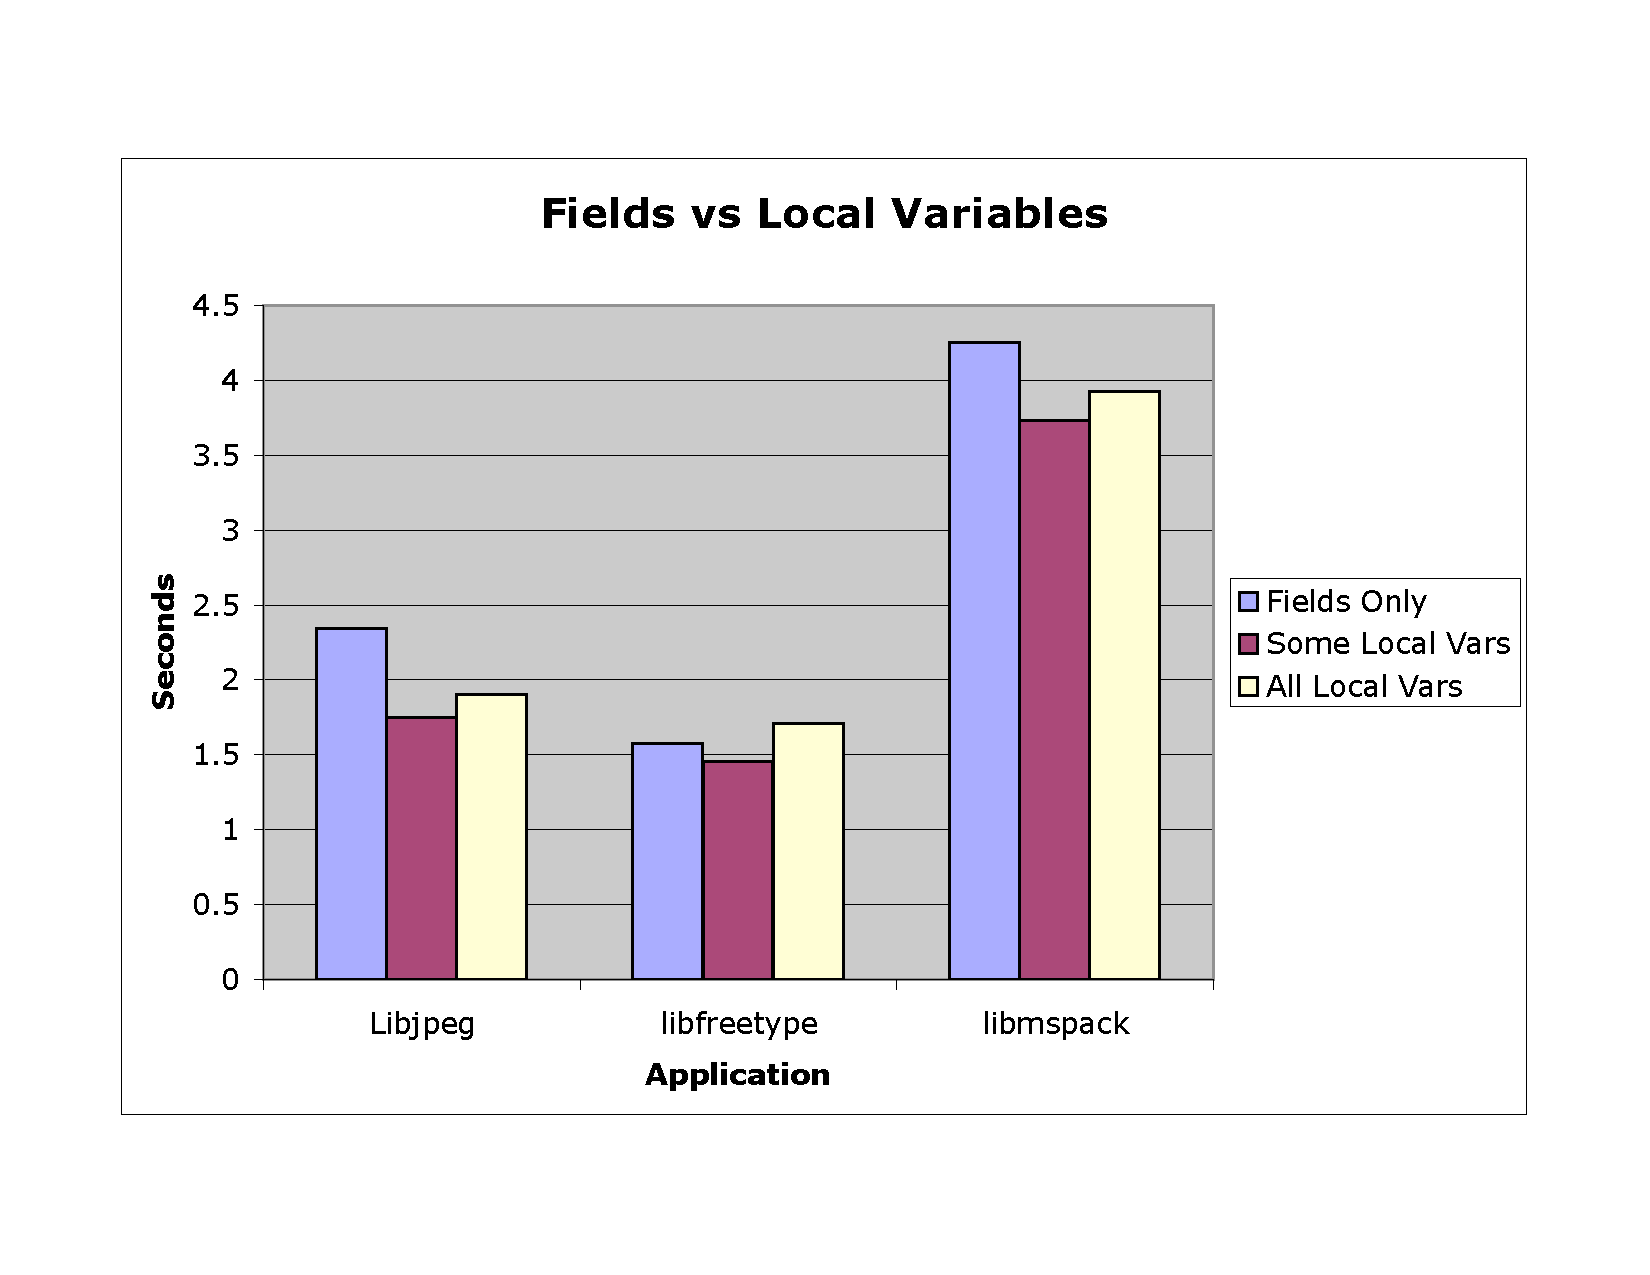
\epsfig{file=chart1,width=3in}

Unfortunately, Java imposes a 64kb limit on the size of the bytecode
for a single method.  This presents a problem for NestedVM, and
necessitates a {\it trampoline transformation}, as shown in
Figure~\ref{code1}.  With this trampoline in place, large binaries can
be handled without much difficulty -- fortunately, there is no
corresponding limit on the size of a classfile as a whole.

One difficulty that arose as a result of using the trampoline
transformation was the fact that {\tt javac} and {\tt jikes} are
unable to properly optimize its switch statements.  For example, the
following code is compiled into a comparatively inefficient {\tt
LOOKUPSWITCH}:

{\footnotesize
\begin{verbatim}
    switch(pc&0xffffff00) {
        case 0x00000100: run_100(); break;
        case 0x00000200: run_200(); break;
        case 0x00000300: run_300(); break;
    }
\end{verbatim}}

\begin{figure}
{\footnotesize\begin{verbatim}
switch(pc>>>8) {
    case 0x1: run_100();
    case 0x2: run_200();
    case 0x3: run_300();
}
\end{verbatim}}

Javac isn't smart enough to see the pattern in the case values and
generates very suboptimal bytecode. Manually doing the shifts
convinces javac to emit a tableswitch statement, which is
significantly faster. This change alone nearly doubled the speed of
the compiled binary.

Finding the optimal method size lead to the next big performance
increase.  It was determined through experimentation that the optimal
number of MIPS instructions per method is 128 (considering only power
of two options). Going above or below that lead to performance
decreases. This is most likely due to a combination of two factors.

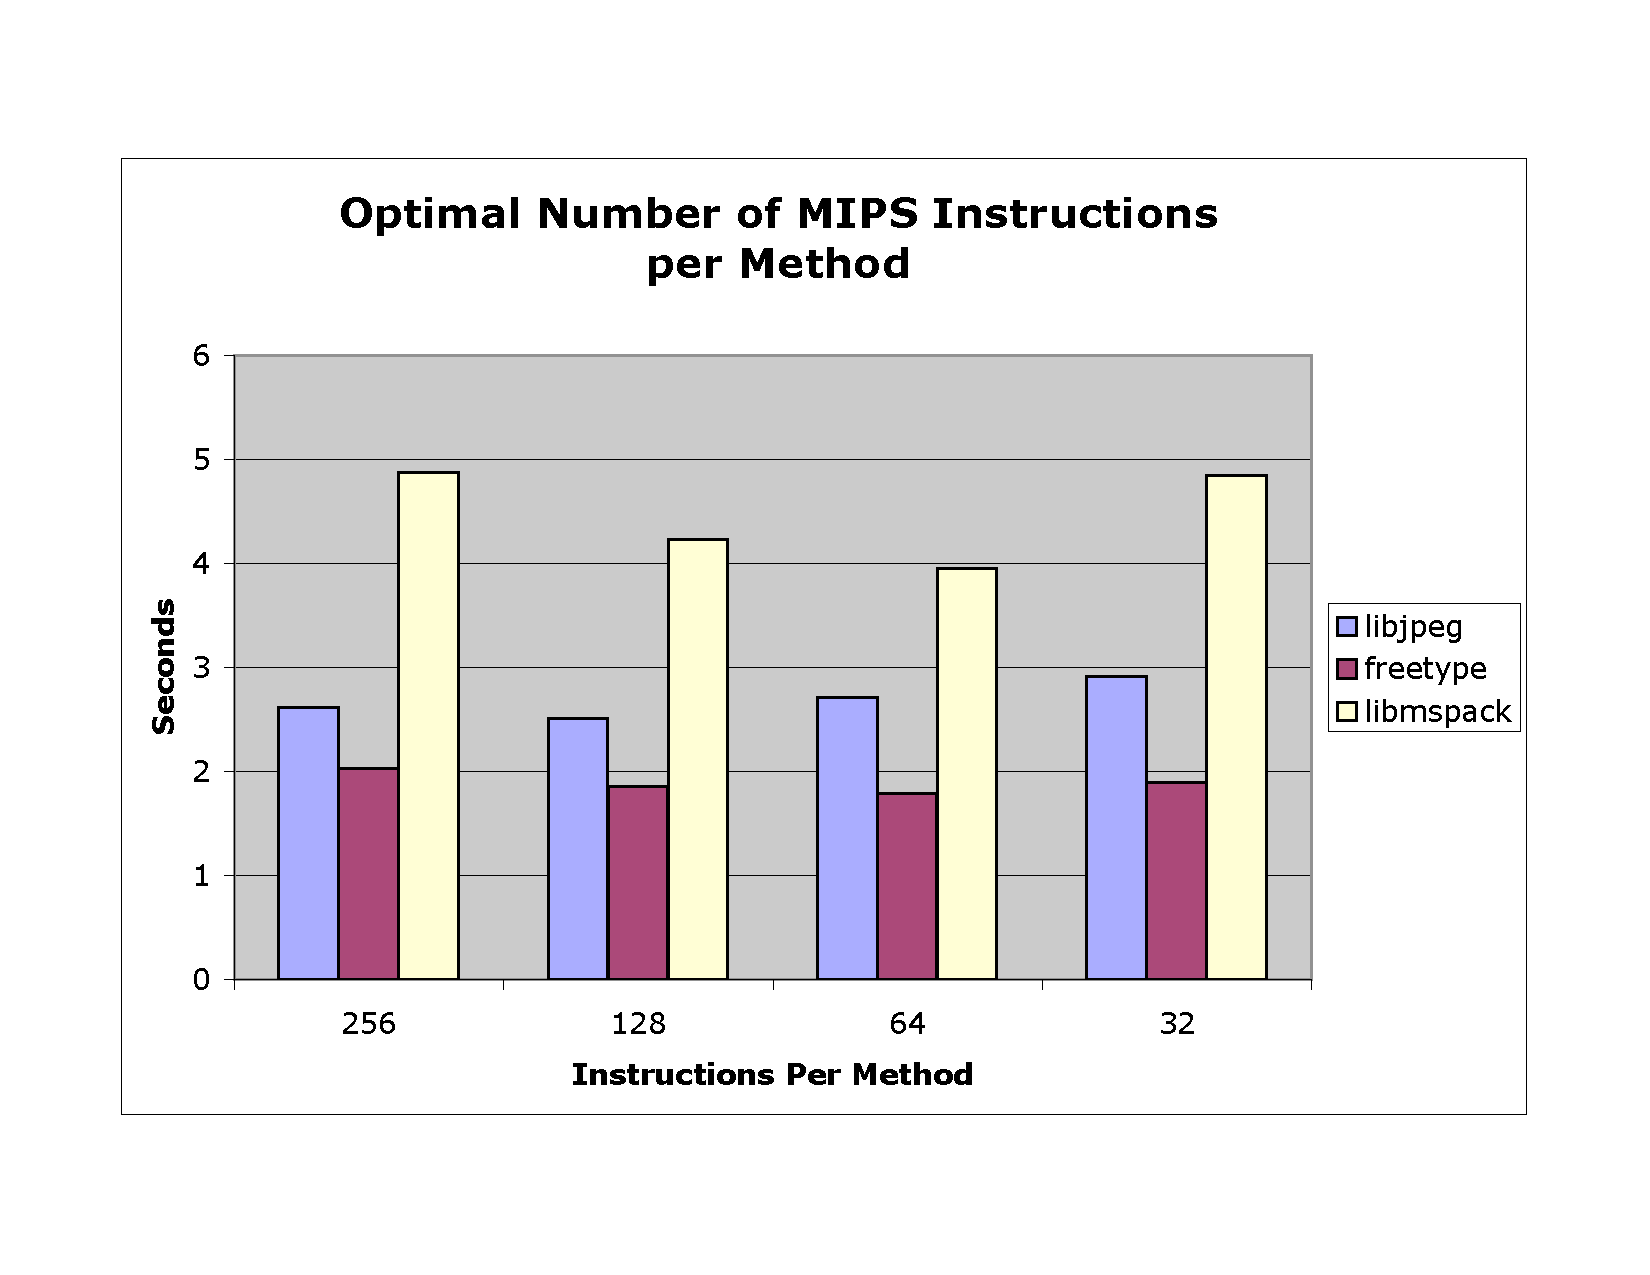
\epsfig{file=chart5,width=3in}

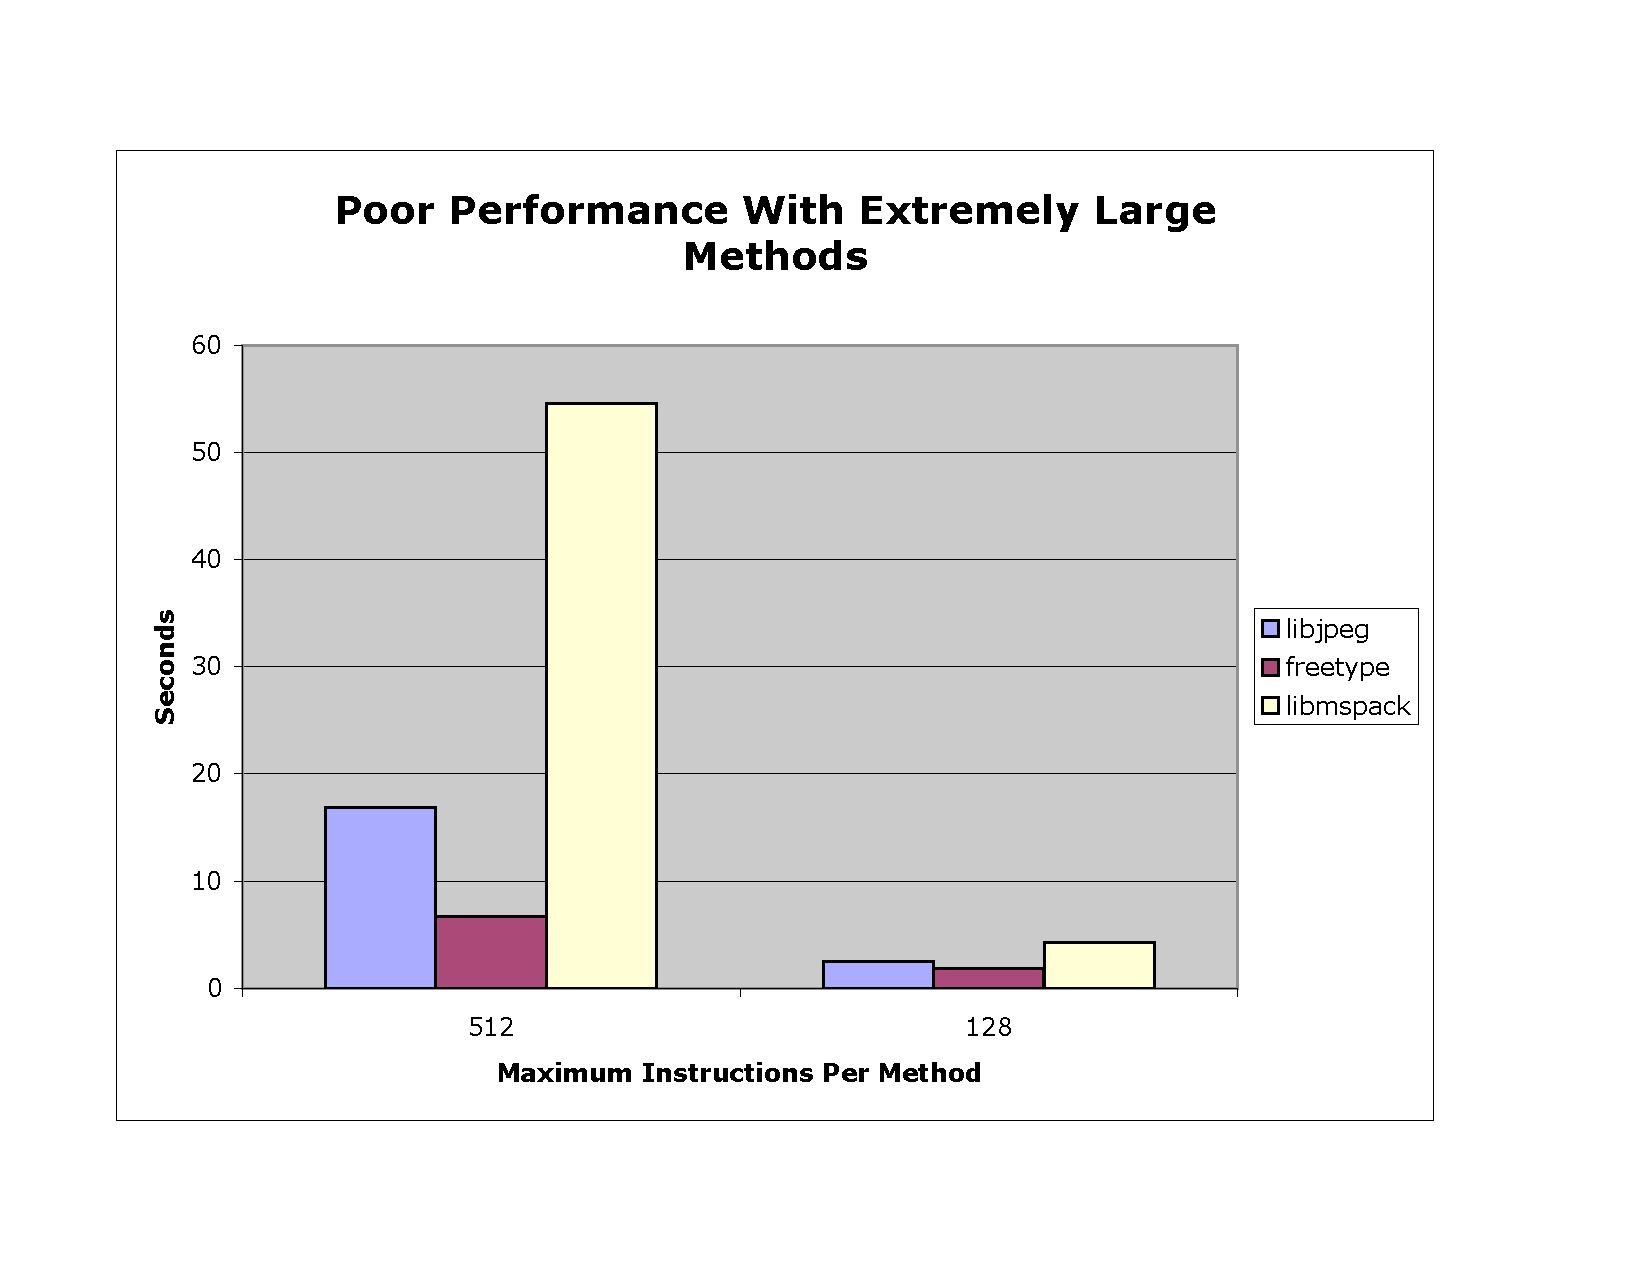
\epsfig{file=chart6,width=3in}

This phenomenon is due to two factors:

\begin{itemize}

\item While the trampoline method's {\tt switch} statement can be
      coded as a {\tt TABLESWITCH}, the {\tt switch} statement
      within the individual methods is to sparse to encode this way.

\item Hybrid Interpretive-JIT compilers such as HotSpot generally
      favor smaller methods since they are easier to compile and are
      better candidates for compilation in ``normal'' programs (unlike
      NestedVM programs).

\end{itemize}

After tuning method sizes, our next performance boost came from
eliminating exraneous case branches.  Having case statements before
each instruction prevents JIT compilers from being able to optimize
across instruction boundaries, since control flow can enter the body
of a {\tt switch} statement at any of the {\tt case}s.  In order to
eliminate unnecessary case statements we needed to identify all
possible jump targets.  Jump targets can come from three sources:

The next big optimization was eliminating unnecessary case
statements. Having case statements before each instruction prevents
JIT compilers from being able to optimize across instruction
boundaries. In order to eliminate unnecessary case statements every
possible address that could be jumped to directly needed to be
identified. The sources for possible jump targets come from 3 places.

\begin{itemize}

\item The .text segment - Every instruction in the text segment is
      scanned for jump targets. Every branch instruction (BEQ, JAL,
      etc) has its destination added to the list of possible branch
      targets. In addition, functions that set the link register have
      theirpc+8 added to the list (the address that would've been put
      to the link register). Finally, combinations of LUI (Load Upper
      Immediate) of ADDIU (Add Immediate Unsigned) are scanned for
      possible addresses in the text segment. This combination of
      instructions is often used to load a 32-bit word into a
      register.

\item The .data segment - When GCC generates switch() statements it
      often uses a jump table stored in the .data
      segment. Unfortunately gcc doesn't identify these jump tables in
      any way. Therefore, the entire .data segment is conservatively
      scanned for possible addresses in the .text segment.
      
\item The symbol table - This is mainly used as a backup. Scanning the
      .text and .data segments should identify any possible jump
      targets but adding every function in the symbol table in the ELF
      binary doesn't hurt. This will also catch functions that are
      never called directly from the MIPS binary (for example,
      functions called with the call() method in the runtime).

      This is mainly used as a backup.  Scanning the {\tt .text} and
      {\tt .data} segments should identify any possible jump targets;
      however, adding all function symbols in the ELF symbol table
      also catches functions that are never called directly from the
      MIPS binary, such as those invoked only via the NestedVM
      runtime's {\tt call()} method.

\end{itemize}

Eliminating unnecessary {\tt case} statements provided a 10-25\% speed
increase.

Despite all the above optimizations, one insurmountable obstacle
remained: the Java {\tt .class} file format limits the constant pool
to 65535 entries.  Every integer literal greater than {\tt 32767}
requires an entry in this pool, and each branch instruction generates
one of these.

One suboptimal solution was to express constants as offsets from a few
central values; for example ``{\tt pc~=~N\_0x00010000~+~0x10}'' (where
{\tt N\_0x000100000} is a non-final field to prevent {\tt javac} from
inlining it).  This was sufficient to get reasonably large binaries to
compile, and caused only a small (approximately 5\%) performance
degredation and a similarly small increase in the size of the {\tt
.class} file.  However, as we will see in the next section, compiling
directly to {\tt .class} files (without the intermediate {\tt .java}
file) eliminates this problem entirely.


\subsection{Binary-to-Binary}

After implementing the binary-to-source compiler, a binary-to-binary
translation mode was added.

\begin{pdfpic}
\newlength{\MyLength}
\settowidth{\MyLength}{xmachine codex}
\newcommand{\MyBox}[1]{\makebox[\MyLength]{#1}}
\psmatrix[colsep=2,rowsep=0,nrot=:U]
  & \\[0pt]
  [name=s0]\MyBox{unsafe source} & [name=s1]\MyBox{safe source}   \\[0pt]
  & \\[0pt]
  & \\[0pt]
  & \\[0pt]
  & \\[0pt]
  & \\[0pt]
  [name=b0]\MyBox{machine code}  & [name=b1]\MyBox{safe bytecode} \\[0pt]
  & \\[0pt]
  \psset{nodesep=5pt,arrows=->}
  \ncline{s0}{b0}\bput{:U}{\tt gcc}
  \ncline{b0}{b1}\naput{\tt NestedVM}
\endpsmatrix
\end{pdfpic}

This mode has several advantages:

\begin{itemize}
      
\item There are little tricks that can be done in JVM bytecode that
      can't be done in Java source code.

\item Directly generating {\tt .class} files Eliminates the
      time-consuming {\tt javac} step.

\item Direct compilation to {\tt .class} files opens up the
      interesting possibility of dynamically translating MIPS binaries
      and loading them via {\tt ClassLoader.fromBytes()} {\it at
      deployment time}, eliminating the need to compile binaries ahead
      of time.

\end{itemize}

Most of the performance improvemen where made where in the handling of
branch instructions and in taking advantage of the JVM stack to
eliminate unnecessary {\tt LOAD}s and {\tt STORE}s to local variables.

The first obvious optimization that generating bytecode allows for is the
use of GOTO. Despite the fact that java doesn't have a GOTO keyword a GOTO
bytecode does exist and is used heavily in the code generates by javac.
Unfortunately the java language doesn't provide any way to take advantage of
this. As result of this, jumps within a method were implemented in the
binary-to-source compiler by setting the PC field to the new address and
making a trip back to the initial switch statement.  In the classfile
compiler these jumps are implemented as GOTOs directly to the target
instruction. This saves a costly trip back through the LOOKUPSWITCH
statement and is a huge win for small loops within a method.

The first optimization gained by direct bytecode generation came from
the use of the JVM {\tt GOTO} instruction.  Despite the fact that the
Java {\it language} does not have a {\tt goto} keyword, the VM does in
fact have a corresponding instruction which is used quite heavily by
{\tt javac}.  NestedVM's binary-to-binary mode exploits this
instruction to avoid emitting inefficient {\tt switch..case}
structures.

Related to the {\tt GOTO} instruction is branch statement
optimization.  When emitting source code, NestedVM translates branches
into Java source code like this:

{\footnotesize\begin{verbatim}
    if (condition) {
        pc = TARGET;
        continue;
    }
\end{verbatim}}

This requires a branch in the JVM regardless of whether the MIPS
branch is actually taken. If condition is false the JVM has to jump
over the code to set the PC and go back to the switch block. If
condition is true the JVM has to jump to the switch block. By
generating bytecode directly we can make the target of the JVM branch
statement the actual bytecode of the final destination. In the case
where the branch isn't taken the JVM doesn't need to branch at all.

A side affect of the above two optimizations is a solution to the
excess constant pool entries problem. When jumps are implemented as
GOTOs and direct branches to the target the PC field doesn't need to
be set. This eliminates many of the constant pool entries the java
source compiler requires. The limit is still there however, and given
a large enough binary it will still be reached.

Implementation of the MIPS delay slot offers another opportunity for
bytecode-level optimization.  In order to take advantage of
instructions already in the pipeline, the MIPS ISA specifies that the
instruction after a jump or branch is always executed, even if the
jump/branch is taken.  This instruction is referred to as the ``delay
slot\footnote{Newer MIPS CPUs have pipelines that are much larger than
early MIPS CPUs, so they have to discard instructions anyways}.''  The
instruction in the delay slot is actually executed {\it before} the
branch is taken.  To further complicate matters, values from the
register file are loaded {\it before} the delay slot is executed.

Fortunately there is a very elegent solution to this problem which can
be expressed in JVM bytecode.  When a branch instruction is
encountered, the registers needed for the comparison are pushed onto
the stack to prepare for the JVM branch instruction.  Then, {\it
after} the values are on the stack the delay slot instruction is
emitted, followed by the actual JVM branch instruction.  Because the
values were pushed to the stack before the delay slot was executed, any
changes the delay slot made to the registers are not visible to the
branch bytecode.

One final advantage that generating bytecode directly allows is a
reduction in the size of the ultimate {\tt .class} file.  All the
optimizations above lead to more compact bytecode as a beneficial side
effect; in addition, NestedVM performs a few additional optimizations.

When encountering the following {\tt switch} block, both {\tt javac}
and {\tt jikes} generate redundant bytecode.

{\footnotesize\begin{verbatim}
    switch(pc>>>8) {
        case 0x1: run_1(); break;
        case 0x2: run_2(); break
        ...
        case 0x100: run_100(); break;
    }
\end{verbatim}}

The first bytecode in each case arm in the switch statement is {\tt
ALOAD\_0} to prepare for a {\tt INVOKESPECIAL} call.  By simply
lifting this bytecode outside of the {\tt switch} statement, each {\tt
case} arm shrinks by one instruction.

\subsubsection{Compiler Flags}

Although NestedVM perfectly emulates a MIPS R2000 CPU, its performance
profile is nothing like that of actual silicon.  In particular, {\tt
gcc} makes several optimizations that increase performance on an
actually MIPS CPU but actually decrease the performance of
NestedVM-generated bytecode.  We found the following compiler options
could be used to improve performance:

\begin{itemize}

\item {\tt -falign-functions}

      Normally a function's location in memory has no effect on its
      execution speed.  However, in the NestedVM binary translator,
      the {\tt .text} segment is split on power-of-two boundaries.  If
      a function starts near the end of one of these boundaries, a
      performance critical part of the function winds up spanning two
      Java methods.  Telling {\tt gcc} to align all functions along
      these boundaries decreases the chance of this sort of splitting.

\item {\tt -fno-rename-registers}

      On an actual silicon chip, using additional registers carries no
      performance penalty (as long as none are spilled to the stack).
      However, when generating bytecode, using {\it fewer}
      ``registers'' helps the JVM optimize the machine code it
      generates by simplifying the constraints it needs to deal with.
      Disabling register renaming has this effect.

\item {\tt -fno-schedule-insns}

      Results of MIPS load operations are not available until {\it
      two} instructions after the load.  Without the {\tt
      -fno-schedule-insns} instruction, {\tt gcc} will attempt to
      reorder instructions to do other useful work during this period
      of unavailability.  NestedVM is under no such constraint, so
      removing this reordering typically generates simpler machine
      code.

\item {\tt -mmemcpy}

      Enabling this instruction causes {\tt gcc} to use the system
      {\tt memcpy()} routine instead of generating loads and stores.
      As explained in the next section, the NestedVM runtime
      implements {\tt memcpy()} using {\tt System.arraycopy()}, which
      is substantially more efficient.

NestedVM has two primary ways of executing code, the interpreter, and the binary translators. Both the interpreter and the output from the binary translators sit on top of a Runtime class. This class provides the public interface to both the interpreter and the translated binaries.

The Runtime class does the work that the operating system usually does.
Conceptually the Runtime class can be thought of as the operating system and
its subclasses (translated binaries and the interpreter) the CPU. The
Runtime fulfills 5 primary goals:

The Runtime class does the work that the operating system usually does. Conceptually the Runtime class can be thought of as the operating system and it�s subclasses (translated binaries and the interpreter) the CPU. The Runtime fulfills 5 primary goals:

\item {\tt -fno-delayed-branch} The MIPS CPU has a delay slot (see
      above). Earlier versions of NestedVM didn't efficiently emulate
      delay slots. This option causes GCC to avoid using delay slots
      for anything (a NOP is simply placed in the delay slot). This
      had a small performance benefit. However, recent versions of
      NestedVM emulate delay slots with no performance overhead so
      this options has little effect. Nonetheless, these delay slots
      provide no benefit under NestedVM either so they are avoided
      with this option.

\item Provides a consistent external interface - The method of actually executing the code (currently only translated binaries and the interpreter) can be changed without any code changes to the caller because only Runtime exposes a public interface.

\item Provide an easy to use interface - The interpreter and the output from the binary translators only know how to execute code. The Runtime class provides an easy to use interface to the code. It contains methods to pass arguments to the main() function, read and write from memory, and call individual functions in the binary.

\item Manage the process�s memory - The Runtime class contains large int[] arrays that represent the process`s entire memory space.  Subclasses read and write to these arrays as required by the instructions they are executing.  Subclasses can expend their memory space using the sbrk syscall.

\item Provide access to the file system and streams - Subclasses access the file system through standard UNIX syscalls (read, write,  open, etc). The Runtime manages the file descriptor table that maps UNIX file descriptors to Java RandomAccessFiles, InputStreams, OutputStreams, and sockets.

\item Miscellaneous other syscalls - In additions to those mentioned above the Runtime class implements a variety of other syscalls (sleep, gettimeofday, getpagesize, sysconf, fcntl, etc).

In addition to binary-to-source and binary-to-binary translation,
NestedVM also includes a MIPS binary interpreter.  All three
translation approaches expose the same API to both the translated
binary and the surrounding VM (including peer Java code).

\subsection{The Runtime Class}

The runtime fulfills four roles:

\begin{itemize}
      
\item It provides a simple, consistent external interface.  The method
      of actually executing the code (currently only translated
      binaries and the interpreter) can be changed without any code
      changes to the caller because only runtime exposes a public
      interface.  This includes methods to pass arguments to the
      binary's {\tt main()} function, read and write from memory, and
      call individual functions in the binary.
      
\item It manages the process's memory.  The runtime class contains
      large {\tt int[]} arrays that represent the process`s entire
      memory space.  Subclasses read and write to these arrays as
      required by the instructions they are executing, and can expand
      their memory space using the {\tt sbrk} system call.
      
\item The runtime provides access to the host file system and standard
      I/O streams.  Subclasses of {\tt runtime} can access the file
      system through standard UNIX syscalls ({\tt read()}, {\tt
      write()}, {\tt open()}, etc).  The runtime manages the file
      descriptor table that maps UNIX file descriptors to Java {\tt
      RandomAccessFile}s, {\tt InputStream}s, {\tt OutputStream}s, and
      {\tt Socket}s.
      
\item It provides general OS services, including {\tt sleep()}, {\tt
      gettimeofday()}, {\tt getpagesize()}, {\tt sysconf()}, {\tt
      fcntl()}, and so on.
      
\end{itemize}

\section{Future Directions}

Java source code can create a copy of the translated binary by instantiating the class generated by the binary translator  or instantiating the interpreter. It can then interact with the process through the many facilities provided by the Runtime interface.  Invoking the run() method of the Runtime interface will load the given arguments into the process�s memory as invoke the binaries entry point (typically \_start() in crt0.o). This will pass control on to the main() function which will have the arguments passed to run() loaded into argv and argc.

As the binary executes it often passes control back to the Runtime class through the MIPS {\tt SYSCALL} instruction. The interpreter and translated binaries invoke the {\tt syscall()} method of the Runtime class when the {\tt SYSCALL} instruction is executed. The Runtime class then can manipulate the process�s environment (read and write to memory, modify the file descriptor table, etc) and interact with the rest of the JVM on behalf of the process (read and write to a file or stream, etc). There is even a syscall to pause the VM and temporarily return control to the caller.

In addition to the interfaces provided by NestedVM, users can create their own interfaces between  the MIPS and Java world. The Runtime provides a method called call() that will call a function by name in the MIPS binary. The call() method looks up the function name in the binary�s ELF symbol table and manipulating the stack and registers accordingly to execute the given function. This allows Java code to seamlessly invoke functions in the binary. 

\section{Conclusion}

The MIPS binaries can also invoke a special method of Runtime called callJava().When the MIPS binary invokes the {\tt CALL\_JAVA}  syscall (usually done through the {\tt \_call\_java()} function provided by the NestedVM support library) the callJava() method in Runtime is invoked with the arguments passes to the syscall.

NestedVM is available under an open source license, and can be
obtained from
\begin{verbatim}
    http://nestedvm.ibex.org
\end{verbatim}


\section{Appendix: Testing Methodology}

The MIPS binaries can also invoke a special method of Runtime called
callJava().When the MIPS binary invokes the {\tt CALL\_JAVA} syscall
(usually done through the {\tt \_call\_java()} function provided by
the NestedVM support library) the callJava() method in Runtime is
invoked with the arguments passes to the syscall.

{\footnotesize\begin{verbatim}

// Java
private Runtime rt = new MyBinary() {
    pubilc int callJava(int a, int b, int c, int d) {
        System.err.println("Got " + a + " " + b);
    }
};
public void foo() { rt.run(); }

/* C */
void main(int argc, char **argv) {
    \_call\_java(1,2);
}

\end{verbatim}}

These two methods can even be combined. MIPS can call Java through the CALL\_JAVA syscall, which can in turn invoke a MIPS function in the binary with the call() method.

Users preferring a simpler communication mechanism can also use Java Stream�s and file descriptors. Runtime provides a simple interface for mapping a Java Input or OutputStream to a File Descriptor.

%Java source code can create a copy of the translated binary by
%instantiating the corresponding class, which extends {\tt Runtime}.
%Invoking the {\tt main()} method on this class is equivalent to
%calling the {\tt main()} function within the binary; the {\tt String}
%arguments to this function are copied into the binary's memory space
%and made available as {\tt **argv} and {\tt argc}.

%The translated binary communicates with the rest of the VM by
%executing MIPS {\tt SYSCALL} instructions, which are translated into
%invocations of the {\tt syscall()} method.  This calls back to the
%native Java world, which can manipulate the binary's environment by
%reading and writing to its memory space, checking its exit status,
%pausing the VM, and restarting the VM.


%\subsection{Virtualization}

%The {\tt Runtime} class implements the majority of the standard {\tt
%libc} syscalls, providing a complete interface to the filesystem,
%network socket library, time of day, (Brian: what else goes here?).

%\begin{itemize}

%\item ability to provide the same interface to CNI code and
      % NestedVMified code
      
%\item security advantages (chroot the {\tt fork()}ed process)
      %
%\end{itemize}


\section{Future Directions}

\section{Conclusion}

\section{Appendix A: Testing Environment}

The MIPS binaries can also invoke a special method of Runtime called
callJava().When the MIPS binary invokes the {\tt CALL\_JAVA} syscall
(usually done through the {\tt \_call\_java()} function provided by
the NestedVM support library) the callJava() method in Runtime is
invoked with the arguments passes to the syscall.

Although NestedVM perfectly emulates a MIPS R2000 CPU its performance characteristics aren't anything like an actual MIPS R2000 CPU. GCC makes several optimizations that increase performance on an actually MIPS CPU but actually decrease performance when run through the NestedVM binary translator. Fortunately, GCC provides many options to customize its code generations and eliminate these optimizations. GCC also has optimization options that aren't helpful on a real MIPS CPU but are very helpful under NestedVM

// Java
private Runtime rt = new MyBinary() {
    pubilc int callJava(int a, int b, int c, int d) {
        System.err.println("Got " + a + " " + b);
    }
};
public void foo() { rt.run(); }

/* C */
void main(int argc, char **argv) {
    _call_java(1,2);
}

\item {\tt -falign-functions}
Normally a function's location in memory has no effect on its execution speed. However, in the NestedVM binary translator, the .text segment is split up on power of two boundaries. If a function is unlucky enough to start near the end of one of these boundaries a performance critical part of the function could end up spanning two methods. There is a significant amount of overhead in switching between two methods so this must be avoided at all costs. By telling GCC to align all functions to the boundary that the .text segment is split on the chances of a critical part of a function spanning two methods is significantly reduced.

\item {\tt -fno-rename-registers}
Some processors can better schedule code when registers aren't reused for two different purposes. By default GCC will try to use as many registers as possibly when it can. This excess use of registers just confuses JIT's trying to compile the output from the binary translator. All the JIT compilers we tested do much better with a few frequently used registers.

\item {\tt -fno-delayed-branch}
The MIPS CPU has a delay slot (see above). Earlier versions of NestedVM didn't efficiently emulate delay slots. This option causes GCC to avoid using delay slots for anything (a NOP is simply placed in the delay slot). This had a small performance benefit. However, recent versions of NestedVM emulate delay slots with no performance overhead so this options has little effect. Nonetheless, these delay slots provide no benefit under NestedVM either so they are avoided with this option.

\item {\tt -fno-schedule-insns}
Load operations in the MIPS ISA also have a delay slot. The results of a load operation are not available for use until one instruction later. Several other instructions also have similar delay slots. GCC tries to do useful work wile waiting for the results of one of these operations by default. However, this, like register renaming, tends to confuse JIT compilers. This option prevents GCC from going out of its way to take advantage of these delay slots and makes the code generated by NestedVM easier for JIT compilers to handle.

\item {\tt -mmemcpy}
GCC sometimes has to copy somewhat large areas of memory. The most common example of this is assigning one struct to another. Memory copying can be done far more efficiently in Java than under NestedVM. Calls to the memcpy libc function are treated specially by the binary translator. They are turned into calls to a memcpy method in Runtime. The {\tt -mmemcpy} option causes GCC to invoke libc's memcpy() function when it needs to copy a region of memory rather than generating its own memcpy code. This call in then turned into a call to this Java memcpy function which is significantly faster than the MIPS implementation.

\item {\tt -ffunction-sections -fdata-sections}
These two options are used in conjunction with the {\tt --gc-section} linker option. These three options cause the linker to aggressively discard unused functions and data sections. In some cases this leads to significantly smaller binaries.

%\subsection{Virtualization}

%The {\tt Runtime} class implements the majority of the standard {\tt
%libc} syscalls, providing a complete interface to the filesystem,
%network socket library, time of day, (Brian: what else goes here?).

World domination.

\item Better use of local variables in binary-to-binary compiler -- need to
do data flow analysis to find how how and when registers are used and avoid
the costly load/restore when it isn't necessary.

\item More advanced Runtime support -- support more syscalls. This will
allow running large applications such as GCC under NestedVM.

\item World domination

\end{itemize}

%\item ability to provide the same interface to CNI code and
      % NestedVMified code
      
%\item security advantages (chroot the {\tt fork()}ed process)
      %
%\end{itemize}


\section{Future Directions}

\section{Conclusion}

\section{Appendix A: Testing Environment}

All times are measured in seconds. These were all run on a dual 1Ghz
Macintosh G4 running Apple's latest JVM (Sun HotSpot JDK 1.4.1). Each
test was run 8 times within a single VM. The highest and lowest times
were removed and the remaining 6 were averaged. In each case only the
first run differed significantly from the rest.

The libjpeg test consisted of decoding a 1280x1024 jpeg
(thebride\_1280.jpg) and writing a tga. The mspack test consisted of
extracting all members from arial32.exe, comic32.exe, times32.exe, and
verdan32.exe. The freetype test consisted of rendering characters
32-127 of Comic.TTF at sizes from 8 to 48 incrementing by 4. (That is
about 950 individual glyphs).

\section{References}

\end{document}

